\documentclass[10pt,a4paper]{article}
%\documentclass[12pt,a4paper]{article}

\usepackage[utf8]{inputenc}
\usepackage{hyperref}
\usepackage{polski}
\usepackage{graphicx}
\usepackage{listings}
\usepackage{algorithm}
\usepackage{algorithmic}
\usepackage{array}

\usepackage{hyperref}
%\usepackage{antpolt}
\usepackage{amssymb}
\usepackage{multicol}
\usepackage{fancyvrb}

\usepackage{color}

%\setlength{\topskip}{0mm} \setlength{\footskip}{0mm} \setlength{\topmargin}{0mm} \setlength{\marginparwidth}{0mm}
%\setlength{\headsep}{2mm} \setlength{\headheight}{0mm} \setlength{\textheight}{250mm}
%\setlength{\textwidth}{160mm} \setlength{\oddsidemargin}{0mm} \setlength{\evensidemargin}{0mm}

\setlength{\topskip}{0mm} \setlength{\topmargin}{0mm}
\setlength{\oddsidemargin}{0mm} \setlength{\evensidemargin}{0mm}
\setlength{\marginparwidth}{0mm} \setlength{\headsep}{0mm}
\setlength{\headheight}{0mm} \setlength{\textheight}{240mm}
\setlength{\textwidth}{170mm}


\floatname{algorithm}{Algorytm}
\renewcommand{\lstlistlistingname}{Spis listingów}
\renewcommand{\lstlistingname}{Listing}

\newcommand{\centered}[1]{\begin{tabular}{l} #1 \end{tabular}}

\lstset{literate=
  {á}{{\'a}}1 {é}{{\'e}}1 {í}{{\'i}}1 {ó}{{\'o}}1 {ú}{{\'u}}1
  {Á}{{\'A}}1 {É}{{\'E}}1 {Í}{{\'I}}1 {Ó}{{\'O}}1 {Ú}{{\'U}}1
  {à}{{\`a}}1 {è}{{\`e}}1 {ì}{{\`i}}1 {ò}{{\`o}}1 {ù}{{\`u}}1
  {À}{{\`A}}1 {È}{{\'E}}1 {Ì}{{\`I}}1 {Ò}{{\`O}}1 {Ù}{{\`U}}1
  {ä}{{\"a}}1 {ë}{{\"e}}1 {ï}{{\"i}}1 {ö}{{\"o}}1 {ü}{{\"u}}1
  {Ä}{{\"A}}1 {Ë}{{\"E}}1 {Ï}{{\"I}}1 {Ö}{{\"O}}1 {Ü}{{\"U}}1
  {â}{{\^a}}1 {ê}{{\^e}}1 {î}{{\^i}}1 {ô}{{\^o}}1 {û}{{\^u}}1
  {Â}{{\^A}}1 {Ê}{{\^E}}1 {Î}{{\^I}}1 {Ô}{{\^O}}1 {Û}{{\^U}}1
  {Ã}{{\~A}}1 {ã}{{\~a}}1 {Õ}{{\~O}}1 {õ}{{\~o}}1
  {œ}{{\oe}}1 {Œ}{{\OE}}1 {æ}{{\ae}}1 {Æ}{{\AE}}1 {ß}{{\ss}}1
  {ű}{{\H{u}}}1 {Ű}{{\H{U}}}1 {ő}{{\H{o}}}1 {Ő}{{\H{O}}}1
  {ç}{{\c c}}1 {Ç}{{\c C}}1 {ø}{{\o}}1 {å}{{\r a}}1 {Å}{{\r A}}1
  {€}{{\euro}}1 {£}{{\pounds}}1 {«}{{\guillemotleft}}1
  {»}{{\guillemotright}}1 {ñ}{{\~n}}1 {Ñ}{{\~N}}1 {¿}{{?`}}1
  {ł}{\l{}}1 {ś}{{\'s}}1 {ź}{{\.z}}1  {ó}{{\'o}}1
  {ą}{{\k{a}}}1
}

\begin{document}

\pagestyle{plain}
\begin{center}
\begin{center}
    
\includegraphics[width=.55\textwidth]{logo}
\end{center}
\vspace{0.5cm}
\textsc{\Huge{Uniwersytet Zielonogórski}}\\
\LARGE{Wydział Informatyki, Elektrotechniki i~Automatyki}\\
\large{Instytut Sterowania i Systemów Informatycznych}\\
\vspace{0.5cm}
\Large{Programowanie gier 3D -- Projekt}\\
Prowadzący: Mgr inż. Marcin Skobel \\ 
\vspace{2cm}
\LARGE{Wściekły Maks}\\
\vspace{2cm} 
\Large{Stanisław Mól, Erwin Konkel} \\
\Large{Grupa dziekańska: 33INF-SSI-SP} \\
\vspace{0.5cm} 
\Large{Data oddania projektu: 22.01.2021}
\vspace{4cm}
\begin{flushleft}
	Ocena: ..........................................
\end{flushleft}
\vspace{1cm}
\end{center}

%
% spis treści
%
\footnotesize
\tableofcontents


%
% spis listingów
%
\footnotesize
\lstlistoflistings

\noindent\makebox[\linewidth]{\rule{0.6\paperwidth}{0.4pt}}

\clearpage
\section{Wprowadzenie}
Projekt jest to gra typu przygodowo-bijatykowej o otwartym wielkim świecie. Trafiamy na obszar startowy, w którym pomagają nam postacie w grze i mówią co mamy robić jako zadania w świeci gry. Mapa jest wielką pustynią z charakterystycznymi punktami i trzema wioskami w ktorych otrzymujemy zadania. Polega to na podróżowaniu między wioskami i walce z pojawiającymi się potworami. Platforma sprzętowa to komputery z systemem Windows

\section{Charakterystyka techniczna}
\subsection{Statystyki techniczne}
Całkowita rozmiar gry to 575MB, średnia ilość FPS w grze wacha się pomiędzy 60-90. Najbardziej obciążającą lokalizacją jest wioska "Na prawo". 

\begin{figure}[ht!]
\begin{center}
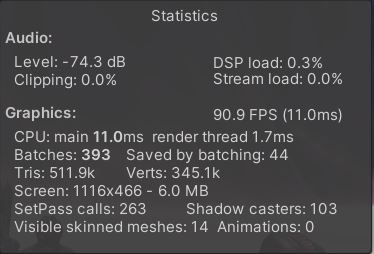
\includegraphics[width=0.8\textwidth]{pictures/FPS_LOW_LOCATION.jpg}
\end{center}
\caption{Statystyki gry.}
\end{figure}

\subsection{Najciekawsze rozwiązania techniczne zastosowane w grze}
\subsubsection{Skrypty}
\begin{lstlisting}[caption={Skrypt 'Timer' - wykonywanie akcji po ustawionym uprzednio czasie}]
using UnityEngine;
using UnityEngine.Events;
using System;
using System.Collections;

public enum TimerMode
{
    CountToDown,
    CountToUp
};

public class Timer : MonoBehaviour
{


    public float timerCounter;
    public float timerTarget;
    public bool isRun;
    public TimerMode timerMode;
    public UnityEvent OnTimerComplete;
    public UnityEvent OnTimerCount;


    public void InitializeTimer(float startValue, float targetValue, TimerMode mode)
    {
        try
        {
            setTimerCounter(startValue);
            setTimerMode(mode);
            setTimerTarget(targetValue);
        }
        catch (ArgumentException)
        {
            Debug.Log("Initialize Timer had set invalid parameters!");
        }
    }

    public void run()
    {
        isRun = true;
    }

    public void stop()
    {
        isRun = false;
    }


    private void Update()
    {
        if (isRun)
        {

            OnTimerCount.Invoke();

            bool condition = false;

            if (timerMode == TimerMode.CountToUp)
            {
                condition = (timerCounter > timerTarget) ? true : false;
                timerCounter += Time.deltaTime;
            }
            else
            {
                condition = (timerCounter < timerTarget) ? true : false;
                timerCounter -= Time.deltaTime;
            }

            if (condition == true)
            {

                stop();
                OnTimerComplete.Invoke();
            }

        }

    }

    public void setTimerCounter(float timerCounter)
    {

        if (timerCounter == 0)
        {
            throw new ArgumentException("Time must be greater than 0!", "timerCounter");
        }

        this.timerCounter = timerCounter;
    }

    public float getTimerCounter()
    {
        return timerCounter;
    }

    public void setTimerTarget(float timerTarget)
    {
        if (timerTarget < 0)
        {
            throw new ArgumentException("Timer duration must be greater than 0!", "timerDuration");

        }

        this.timerTarget = timerTarget;
    }

    public float getTimerTarget()
    {
        return timerTarget;
    }

    public void setTimerMode(TimerMode timerMode)
    {

        if (!Enum.IsDefined(typeof(TimerMode), timerMode))
        {
            throw new ArgumentException("Mode of Timer must set right!", "timerCountMode");
        }

        this.timerMode = timerMode;
    }

    public TimerMode getTimerCountMode()
    {
        return timerMode;
    }

    public void ResetTimer()
    {
        timerCounter = 0;
    }

}
\end{lstlisting}

\begin{lstlisting}[caption={Skrypt 'EnemyAi' - zachowanie oraz poruszanie się przeciwników}]
using System.Collections;
using System.Collections.Generic;
using UnityEngine;
using UnityEngine.AI;

public class EnemyAi : MonoBehaviour
{

    public int health = 100;
    public NavMeshAgent agent;
    public Transform player;
    public LayerMask whatIsGrounde, whatIsPlayer;

    public Vector3 walkPoint;
    bool walkPointSet;
    public float walkPointRange;

    public float timeBetweenAttacks;
    bool alreadyAttacked;
    public GameObject projectile;

    public float sightRange, attackRange;
    public bool playerInSightRange, playerInAttackRange;

    public Animator animator;

    private void Awake()
    {
        agent = GetComponent<NavMeshAgent>();
        player = GameObject.FindGameObjectWithTag("Player").transform;
    }

    private void SearchWalkPoit()
    {
        float randomZ = Random.Range(-walkPointRange, walkPointRange);
        float randomX = Random.Range(-walkPointRange, walkPointRange);

        walkPoint = new Vector3(transform.position.x + randomX, transform.position.y, transform.position.z + randomZ);

        if (Physics.Raycast(walkPoint, -transform.up, 2f, whatIsGrounde))
            walkPointSet = true;
    }

    private void Patroling()
    {
        animator.SetBool("isAttack", false);
        animator.SetBool("isDead", false);

        if (!walkPointSet) SearchWalkPoit();
        if (walkPointSet) agent.SetDestination(walkPoint);

        Vector3 distanceToWalkPoint = transform.position - walkPoint;

        if (distanceToWalkPoint.magnitude < 1f) walkPointSet = false;
    }

    private void ChasePlayer()
    {
        agent.SetDestination(player.position);
    }

    private void AttackPlayer()
    {
        animator.SetBool("isAttack", true);
        agent.SetDestination(transform.position);
        transform.LookAt(player);

        if(!alreadyAttacked)
        {
            alreadyAttacked = true;
            Invoke(nameof(ResetAttack), timeBetweenAttacks);
            RaycastHit theHit;

            if (Physics.Raycast(transform.position, transform.TransformDirection(Vector3.forward), out theHit))
            {
                theHit.transform.SendMessage("HitByEnemy");
            }
        }
    }

    private void ResetAttack()
    {
        animator.SetBool("isAttack", false);
        alreadyAttacked = false;
    }

    private void TakeDamage(int damage)
    {
        health -= damage;
        if (health <= 0) Invoke(nameof(DestroyEnemy), 0.5f);

    }

    private void DestroyEnemy()
    {
        animator.SetBool("isAttack", false);
        animator.SetBool("isDead", true);
    }

    void Update()
    {
        playerInSightRange = Physics.CheckSphere(transform.position, sightRange, whatIsPlayer);
        playerInAttackRange = Physics.CheckSphere(transform.position, attackRange, whatIsPlayer);

        if (!playerInSightRange && !playerInAttackRange) Patroling();
        if (playerInSightRange && !playerInAttackRange) ChasePlayer();
        if (playerInSightRange && playerInAttackRange) AttackPlayer();
    }
}

\end{lstlisting}

\subsubsection{Animator}

\begin{figure}[ht!]
\begin{center}
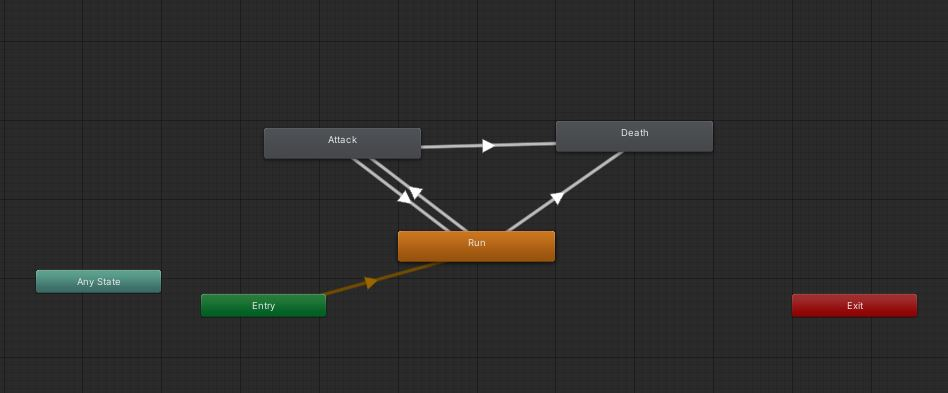
\includegraphics[width=0.8\textwidth]{pictures/EnemyAnimator.jpg}
\end{center}
\caption{Animator - EnemyController}
\end{figure}

\section{Scenariusz gry}
Wcielamy się w rolę fałszywie oskarżonego łowcy przygód, który w trakcie jednej ze swoich wypraw zostaje złapany przez straż panującą w tej krainie. W trakcie ucieczki gubi straż i natrafia na pustynię, na której znajduje obóz w którym wykończony mdlejesz. Okazuje się, że jest to obóz ludzi ktorzy również mają z prawem na pieńku. Po obudzeniu się wita nas kapitan obozu, który daje nam pierwsze zadanie abyśmy dotarli do mędrca w wiosce na wschód. Po drodze atakują nas potwory, które władza wysyła w to miejsce, ponieważ nie potrafi nic innego z nimi zrobić. Okazuje się, że nasze dłonie są magiczne i jesteśmy w stanie te potwory pokonać. W trakcie podróży musimy walczyć o przetrwanie i wydostać się z tej krainy aby udowodnić swoją niewinność. Na końcu spotykamy straszną zjawę, która okazuje się być źródłem powstawania potworów. Kiedy ją pokonujemy, kraina zostaje uratowana i wszyscy mogą spokojnie żyć.

\clearpage
\section{Rozgrywka}

\clearpage
\section{Opis wkładu własnego w realizację projektu}

\vspace{0.5cm}
\begin{description}
  \item[Stanisław Mól:] \hfill
  	\begin{itemize}
 	  \item Postać gracza
 	  \item Poruszanie się gracza
	  \item Pierwszy przeciwnik
	  \item Teren poruszania się przeciwnika
	  \item System animacji przeciwnika
	  \item Atakowanie / poruszanie się przeciwnika (pojawiły się błędy)
	  \item Naprawa błędów
	  \item Zmiana przeciwnika na Humanoidalnego
	  \item Dodanie MainMenu
	\end{itemize}
  \item[ Erwin Konkel:] \hfill
  	\begin{itemize}
          \item Skybox
  	  \item Design mapy
 	  \item Tekstury
  	  \item Wieże
	  \item Wioska początkowa
 	  \item Granice mapy
  	  \item Ulepszenie ścieżki 
  	  \item Poprawione oświetlenie
	  \item Rozwijanie wioski
	  \item NPC
	  \item Dodanie nowego poziomu (nowa wioska)
	\end{itemize}
\end{description}

\clearpage
\section{Spis zastosowanych assetów z krótką charakterystykę}
\begin{itemize}
  \item Third Person Controller - Basic Locomotion FREE - https://assetstore.unity.com/packages/tools/utilities/third-person-controller-basic-locomotion-free-82048
  \item Free Low Poly Desert Pack - https://assetstore.unity.com/packages/3d/environments/free-low-poly-desert-pack-106709
  \item Fantasy Skybox Free - https://assetstore.unity.com/packages/2d/textures-materials/sky/fantasy-skybox-free-18353
  \item Ruined Tower Free - https://assetstore.unity.com/packages/3d/environments/ruined-tower-free-66495
  \item Spider Green - https://assetstore.unity.com/packages/3d/characters/animals/insects/spider-green-11869
  \item Campfire Pack - https://assetstore.unity.com/packages/3d/environments/fantasy/campfire-pack-11256
\end{itemize}

\clearpage
\section{Podsumowanie}
opisanie trudności oraz rozwiązania, wskazanie pozytywnych cech projektu oraz ewentualnych planów i szans na dalszy rozwój projektu.


\noindent\makebox[\linewidth]{\rule{0.6\paperwidth}{0.4pt}}
\begin{center}
	Koniec dokumentu.
\end{center}
\end{document}
